% Greeks Engine -- preparation guide for the project review (explanation, figures, likely questions).
% Build: pdflatex presentation_prep.tex (twice). Figures are the paper's (docs/paper/figures).
\documentclass[11pt,a4paper]{article}
\usepackage[T1]{fontenc}
\usepackage[utf8]{inputenc}
\usepackage{lmodern}
\usepackage[a4paper,margin=2.1cm]{geometry}
\usepackage{graphicx}
\usepackage{booktabs}
\usepackage{array}
\usepackage{amsmath,amssymb}
\usepackage{xcolor}
\usepackage{enumitem}
\usepackage{float}
\usepackage{caption}
\usepackage[colorlinks=true,linkcolor=blue!50!black,urlcolor=blue!50!black]{hyperref}
\setlist{nosep,leftmargin=*,topsep=2pt}
\newcolumntype{L}[1]{>{\raggedright\arraybackslash}p{#1}}
\definecolor{qbg}{HTML}{EEF4FA}
\newcommand{\say}[1]{\par\smallskip\noindent\colorbox{qbg}{\parbox{\dimexpr\linewidth-2\fboxsep}{\textbf{Say:} #1}}\par\smallskip}
\newcounter{qn}
\newcommand{\qa}[2]{\stepcounter{qn}\par\medskip\noindent\textbf{Q\theqn. #1}\par\noindent #2\par}
\graphicspath{{../paper/figures/}}

\title{\textbf{Greeks Engine: Preparation Guide for the Project Review}\\[3pt]
\large The project explained, the figures that go into the paper, and the questions to expect}
\author{Yash Agrawal \quad $\cdot$ \quad BITS Pilani}
\date{27 October 2026}

\begin{document}
\maketitle
\tableofcontents
\bigskip

% =====================================================================
\section{The project in two minutes}
\textbf{What it is.} An FPGA engine that computes the price of a European option under the
\textbf{Heston stochastic-volatility model} together with \textbf{all nine sensitivities
(Greeks)} in one pass, using \textbf{adjoint (reverse-mode) differentiation} built directly
into a fixed-point hardware datapath.

\textbf{Why it matters.} Greeks drive hedging and risk. The industry default on hardware is
\emph{bump-and-reprice}: change one input, price again. Nine Greeks by central differences
cost 19 pricings, and their accuracy depends on an arbitrary bump size. In software, adjoint
differentiation is the standard alternative, but it records a ``tape'' and costs about 5--8
pricings in practice. \textbf{No published FPGA work computes Greeks by an adjoint.}

\textbf{The key idea.} The COS pricing method performs exactly the same operations for every
input. So the reverse sweep can be written once, scheduled at design time into the same
datapath as the forward pass, with no tape memory and no replay logic, and its
multiplications fill multiplier slots the forward pass leaves idle.

\textbf{Headline results.}
\begin{itemize}
\item Price + 9 Greeks for \textbf{1.04$\times$} the cycles of the price alone on the same hardware
(4,733 vs.\ 4,568); against a price-only engine of the \emph{same throughput} (half the multipliers),
\textbf{1.03$\times$ the cycles, 1.68$\times$ the LUTs, 2$\times$ the DSPs} (Vivado). Bump-and-reprice needs
18.4$\times$ more cycles on the same hardware.
\item \textbf{No speed or energy advantage over a well-optimised CPU}: vectorised analytic Greeks take
13.6\,$\mu$s on one laptop core (ZCU102 engine: 15.9\,$\mu$s computed), and energy is at parity
(40 vs.\ 40.9\,$\mu$J, CPU package power measured).
\item A \textbf{first-order rounding-error bound} for every Greek, never exceeded: worst 0.378 of
the bound over 10,500 inputs, 0.356 on a held-out 10,500, $\le$ 0.255 on silicon.
\item \textbf{Bit-exact on two FPGA families}: ZedBoard (Zynq-7020) 450/450; ZCU102 (Zynq
UltraScale+) 1,010/1,010, including 50 real NIFTY market calibrations.
\item \textbf{One generator} produces everything from one description: bit-accurate model,
error bound, scheduled Verilog, bus wrappers and host C code.
\end{itemize}

% =====================================================================
\section{The mathematics you must be able to defend}
\subsection{Heston model}
Under the risk-neutral measure:
$\mathrm{d}S = rS\,\mathrm{d}t + \sqrt{v}\,S\,\mathrm{d}W_1$,\quad
$\mathrm{d}v = \kappa(\theta - v)\,\mathrm{d}t + \xi\sqrt{v}\,\mathrm{d}W_2$,\quad
$\mathrm{d}W_1\mathrm{d}W_2 = \rho\,\mathrm{d}t$.

Nine inputs: $S_0$ spot, $K$ strike, $T$ maturity, $r$ rate, $v_0$ initial \emph{variance},
$\kappa$ mean-reversion speed, $\theta$ long-run variance, $\xi$ vol-of-vol, $\rho$
correlation. No closed-form price, but the \textbf{characteristic function} of $\log S_T$ is
known. We use the numerically stable form (Albrecher et al., ``the little Heston trap''),
which avoids the branch-cut discontinuity of the complex logarithm.

\subsection{The COS method (Fang \& Oosterlee, 2008)}
Truncate the log-price density to $[a,b]$, expand it in a cosine series whose coefficients
come straight from the characteristic function:
\[
V \approx K e^{-rT} {\sum_{k=0}^{N-1}}{}^{\prime} \mathrm{Re}\!\left[\varphi(u_k)\,e^{iu_k(x-a)}\right] U_k,
\qquad u_k = \frac{k\pi}{b-a}.
\]
Our choices: $N = 128$ terms; range $c_1 \pm 10\sqrt{c_2}$ from the cumulants (``$\pm$10
standard deviations''); the range is \textbf{held fixed} when differentiating, so the Greeks
are exact derivatives of the COS approximation at a fixed range (the reference uses the same
convention). We \textbf{price puts and get calls by put--call parity}
$C = P + S_0 - Ke^{-rT}$: call payoff coefficients grow like $e^{b}$ and cancel badly in
fixed point; parity made the worst call price error 75$\times$ smaller.
\textbf{The 128 terms are independent of each other}: the hardware pipelines them.

\subsection{The Greeks we compute}
Delta $\partial V/\partial S_0$; strike sensitivity $\partial V/\partial K$; theta
$\partial V/\partial T$; rho $\partial V/\partial r$; vega $\partial V/\partial v_0$ (with
respect to \emph{variance}; $\partial V/\partial\sigma_0 = 2\sigma_0\,\partial V/\partial v_0$);
and the model-parameter sensitivities $\partial V/\partial\kappa$, $\partial V/\partial\theta$,
$\partial V/\partial\xi$, $\partial V/\partial\rho$, used in calibration and model risk.

\subsection{Adjoint (reverse-mode) differentiation}
Forward (tangent) mode pushes one input direction through the computation: one sweep per
input, nine here. Reverse (adjoint) mode pushes the sensitivity of \emph{one output}
backwards and yields all input derivatives at once; the ``cheap gradient principle'' says
this costs a small constant multiple of the function (theory: $\le$ 4--5$\times$).

In software the forward values needed by the backward sweep are stored on a \textbf{tape},
which is memory-bound: 5.7--7.6 pricings on our CPU (CoDiPack 7.6). In our engine there is
\textbf{no tape memory}: control flow never depends on the input, so every forward value's
lifetime is known at design time, and the scheduler keeps it in a rotating register exactly as
long as the reverse sweep needs it. It is a \emph{register-resident tape compiled into the
schedule}: 447 rotating registers across all terms in flight (the price-only schedule needs 150),
which is why the Greeks add 11,901 flip-flops in Vivado. Say ``register-resident tape'', not
``tape-free''.

\textbf{State this yourself:} the reverse sweep is \textbf{hand-derived} as operations in the
generator's graph (\texttt{heston.py}) and verified numerically. The generator does not
differentiate automatically yet. The claim is ``adjoint differentiation'', not
``\emph{automatic} adjoint differentiation''; ``aad'' in module names is historical.

\subsection{Fixed point and the first-order error bound}
Every value is an integer $\times\,2^{-FL}$: the ZedBoard design uses 56-bit words with 28
fraction bits (Q28), the 64-bit design 64-bit words with 32 (Q32). Round-to-nearest after
every operation, so each rounding contributes at most $\tfrac12$ ulp $= 2^{-(FL+1)}$.

The bound (Linnainmaa 1976, first order):
\[
|\text{error in output } y| \le \sum_{\text{rounding nodes } i}
\left|\frac{\partial y}{\partial w_i}\right| \cdot 2^{-(FL+1)} .
\]
The sensitivities $\partial y/\partial w_i$ come from a reverse sweep over the graph.
Products of two rounding errors (second order, $\approx 2^{-28}$ smaller) are dropped. It
covers \textbf{rounding only}, against the same algorithm computed exactly; the COS method's
own truncation error is a separate term. The bound is computed \textbf{in software} by the
model (0.1\,s per parameter set); the hardware does not output it. Two checks justify
dropping second-order terms: a 50-digit evaluation (hardware error $\le$ 0.24 of the bound)
and the 44-bit design (second-order terms 4,096$\times$ larger), where the bound still held.

% =====================================================================
\section{Architecture and how it works}
\subsection{The generator (\texttt{hardware/gen/})}
\begin{center}\small
\begin{tabular}{@{}L{3.6cm}L{11.8cm}@{}}
\toprule
\textbf{Module} & \textbf{Job}\\
\midrule
\texttt{heston.py} & Builds the operation graph: setup (once), term $k$ ($\times$128) including the reverse sweep, finish (once). Bit-accurate emulator.\\
\texttt{ir.py} & Graph representation; fixed-point and double evaluation; the error bound.\\
\texttt{prims.py} & Newton--Raphson reciprocal and sqrt (table seeds), Tang's exponential, log (table + series), CORDIC rotation/vectoring. No dividers.\\
\texttt{ranges.py} & Measures the data-dependent shift ranges over the input domain (with margin); shifters built only that wide.\\
\texttt{sched.py} & Modulo scheduler: shares 8 multipliers and 5 CORDIC units across overlapping terms.\\
\texttt{rtlgen.py} & Emits the Verilog.\\
\texttt{wrappers.py} & AXI4-Lite / AXI-Stream register-file wrappers.\\
\texttt{host.py}, \texttt{cgen.py} & Host setup/finish steps in Python and as bit-exact generated C (ARM).\\
\texttt{tangent.py} & The three forward-mode baselines (dense, sparse, factored).\\
\texttt{check\_accuracy.py}, \texttt{board\_vectors.py}, \texttt{chain.py} & Accuracy checks, board test vectors, strike-chain study.\\
\bottomrule
\end{tabular}
\end{center}
Because the RTL and the model come from the same graph, the testbench checks \textbf{every
register at the cycle it becomes valid} (1,213--1,962 checks per design), so the hardware
inherits every property shown for the model.

\subsection{Inside the engine}
\begin{itemize}
\item Per evaluation: \textbf{setup} once (characteristic-function constants, truncation
range), \textbf{128 terms} (forward pass, then its reverse sweep), \textbf{finish} once
(discounting, final chain rule, put--call parity).
\item Per term: forward pass (payoff coefficient, characteristic function) $\rightarrow$ reverse
sweep back to the inputs (reusing the forward reciprocals) $\rightarrow$ power-of-two
normalisation (keeps tiny adjoints of high-frequency terms at full precision) $\rightarrow$
nine accumulators.
\item Each term costs exactly \textbf{250 multiplications, 3 CORDIC rotations, 2 CORDIC
vectorings} (the price alone: 126 multiplications).
\item Resources: 8 shared multipliers, 3 rotation and 2 vectoring units. Initiation interval:
$\lceil 250/8\rceil = 32$, $3\cdot 32/3 = 32$, $2\cdot 32/2 = 32$: all three balance at
\textbf{II = 32}. One term lasts 506 cycles, so about 16 terms are in flight. Loop:
$127\times32 + 506 + 2 = $ \textbf{4,572 cycles}; fully on chip (\texttt{z7}): \textbf{4,733}.
\item \textbf{Why the Greeks are nearly free:} the CORDIC units set the pace, so in every
32-cycle window the forward pass leaves multiplier slots idle; the reverse sweep's
multiplies fill them.
\item A 56$\times$56-bit multiplier is built from 9 DSP48 blocks (25$\times$18 each): 8
multipliers = 72 DSPs.
\item Shifters cut to measured ranges saved 35\% of logic; an input that would exceed a range
raises \texttt{range\_err} instead of returning a wrong value; no valid input raises it after
the refit at the domain edges.
\end{itemize}

\subsection{Three configurations (never mix their numbers)}
\begin{center}\small
\begin{tabular}{@{}lL{5.2cm}rL{4.6cm}@{}}
\toprule
\textbf{Name} & \textbf{What} & \textbf{Cycles} & \textbf{Where it ran}\\
\midrule
\texttt{z7} & 56-bit, everything on chip & 4,733 & simulated (too large with setup/finish for the Zynq-7020)\\
\texttt{z7h} & 56-bit, setup and finish on the host, loop on the FPGA & 4,572 (65.3\,$\mu$s at 70\,MHz) & \textbf{ZedBoard silicon}\\
\texttt{zu} & 64-bit, 32 multipliers, everything on chip & 1,593 (15.9\,$\mu$s at 100\,MHz) & \textbf{ZCU102 silicon}\\
\bottomrule
\end{tabular}
\end{center}

\subsection{Board systems}
\begin{enumerate}
\item \textbf{ZedBoard JTAG system}: Vivado drives the engine over the JTAG cable (JTAG-to-AXI
master $\rightarrow$ AXI4-Lite), no processor software: \textbf{450/450 bit-exact}.
\item \textbf{ZedBoard processor system}: the ARM Cortex-A9 runs setup and finish as
generated C and times each stage. Built; board run pending.
\item \textbf{ZCU102 JTAG system}: the 64-bit engine: \textbf{1,010/1,010 bit-exact}.
\item \textbf{ZCU102 processor system}: the Cortex-A53 times the bus transfers and reads the
board's INA226 power monitors. Built (timing met, +1.772\,ns). The lab board's DDR does not
calibrate with Vivado's preset, so the program now runs from on-chip memory and the setup
skips the DDR steps; \textbf{this run is still pending}.
\end{enumerate}

% =====================================================================
\section{The figures in the paper and how to explain them}
The paper (\texttt{docs/paper/greeks\_engine\_ieee.pdf}) has ten figures, in IEEE style.
Below, in order of importance, is each figure with how to read it and what to say.

\subsection*{Fig.~1 -- Design flow (diagram)}
One operation graph (setup / term / finish) branches into the bit-accurate model, the
double-precision model, the error bound and the modulo scheduler $\rightarrow$ Verilog; the RTL
is checked register by register, implemented in Vivado, run on two boards, and the board
outputs are compared bit for bit with the model.
\say{Because everything comes from one graph, the hardware is correct by construction relative
to the model, and the bound applies to the hardware.}

\subsection*{Fig.~2 -- One COS term and the modulo schedule (diagram)}
Top: forward pass $\rightarrow$ reverse sweep $\rightarrow$ normalisation $\rightarrow$ 9
accumulators, one datapath; forward values held in 447 registers. Bottom: bars 506 cycles long
starting every 32 cycles; about 16 overlap.
\say{The forward values the reverse sweep needs sit in scheduled registers, not in tape memory.
II = 32 is set equally by the multipliers and the CORDIC units; the reverse sweep fits into the
idle multiplier slots because the engine has twice the multipliers a price-only engine needs.}

\begin{figure}[H]\centering
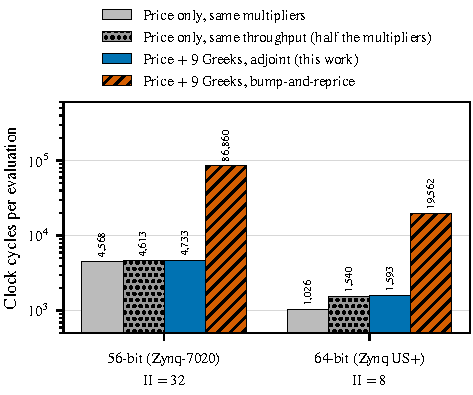
\includegraphics[width=0.62\linewidth]{fig_cycles.pdf}
\caption*{Fig.~3 -- Cycles: price only (same multipliers, and same throughput with half the multipliers), adjoint, bump-and-reprice.}
\end{figure}
\noindent\textbf{How to read it:} log scale. The first two bars are price-only engines: with the
adjoint's multipliers, and with half of them (the same initiation interval, i.e.\ the same
throughput). The adjoint bar is about 3\% above the second on both designs (4,733 vs.\ 4,613;
1,593 vs.\ 1,540); bump-and-reprice is 86,860 and 19,562.
\say{At the same throughput the Greeks cost about 3\% in cycles but twice the multipliers.
Bump-and-reprice needs 18.4$\times$ the cycles on identical hardware.}

\begin{figure}[H]\centering
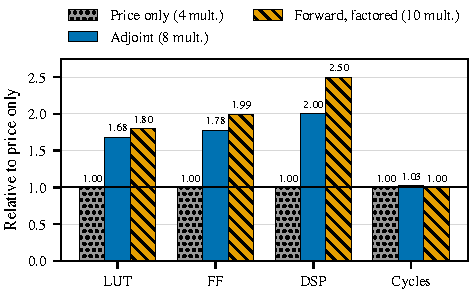
\includegraphics[width=0.62\linewidth]{fig_equal.pdf}
\caption*{Fig.~4 -- Three engines of equal throughput implemented in Vivado, normalised to price only.}
\end{figure}
\noindent\textbf{How to read it:} price only (4 multipliers), adjoint (8), factored forward mode
(10), all at II = 32 on the Zynq-7020. The adjoint costs 1.68$\times$ the LUTs, 1.78$\times$ the
flip-flops and 2$\times$ the DSPs of the price; forward mode costs more on every resource.
\say{This is the real cost of the Greeks: about 1.7$\times$ the area at the same speed. Against a
well-factored forward-mode engine the adjoint saves 7\% of LUTs, 12\% of flip-flops and 20\% of
DSPs and is 6$\times$ more accurate at the same word length. A real but modest advantage.}

\begin{figure}[H]\centering
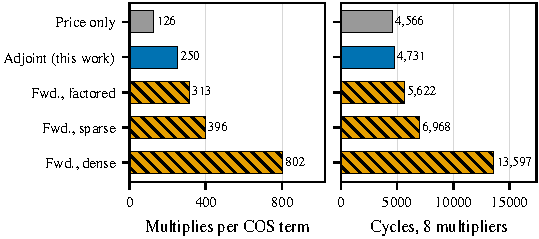
\includegraphics[width=0.62\linewidth]{fig_modes.pdf}
\caption*{Fig.~5 -- Adjoint against three forward-mode datapaths built by the same generator (scheduler).}
\end{figure}
\noindent\textbf{How to read it:} left, multiplies per term (126 price, \textbf{250 adjoint},
313 factored, 396 sparse, 802 dense); right, cycles with 8 multipliers (4,731 vs.\ 5,622,
6,968, 13,597). This is the answer to ``why adjoint and not forward mode?''.
\say{For the same Greeks the adjoint needs the fewest multiplies. To be honest: with 16
multipliers all but the dense one reach $\approx$4,570 cycles, so the 1.04$\times$ is not unique;
what the adjoint saves is \textbf{hardware}: 8 multipliers (72 DSPs) vs.\ 10 (90) for the
factored forward method and 26 (234, more than the chip has) for the dense one.}

\begin{figure}[H]\centering
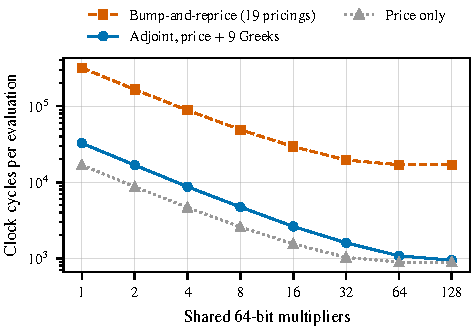
\includegraphics[width=0.62\linewidth]{fig_dse.pdf}
\caption*{Fig.~6 -- Cycles against the number of shared 64-bit multipliers.}
\end{figure}
\noindent\textbf{How to read it:} log--log; cycles halve as multipliers double until the
dependency chain of a term dominates past 64. The adjoint stays 1.1--1.9$\times$ the price and
9.8--18$\times$ below bump-and-reprice throughout.
\say{One generator, one parameter: a small engine for a cheap FPGA or a fast one for a big
FPGA, and the figure shows where extra hardware stops paying.}

\begin{figure}[H]\centering
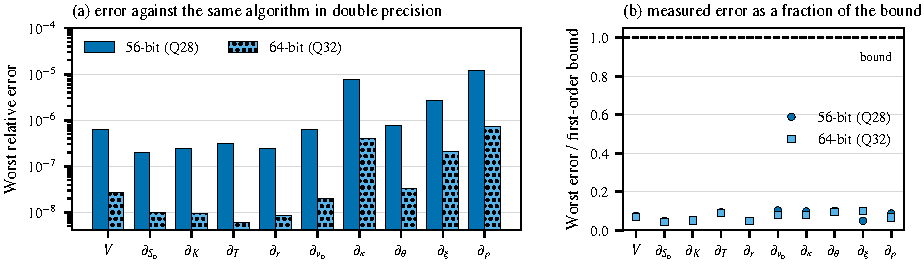
\includegraphics[width=\linewidth]{fig_accuracy.pdf}
\caption*{Fig.~8 -- Accuracy over the 21-case grid: (a) worst relative error, (b) error / bound.}
\end{figure}
\noindent\textbf{How to read it:} (a) 56-bit errors $10^{-7}$ to $1.2\times10^{-5}$, 64-bit
$10^{-8}$ to $7\times10^{-7}$; $\partial_\kappa$ and $\partial_\rho$ are the weakest. (b) every
point is below 0.11, far under the dashed line at 1 (the bound).
\say{Every output stays below its bound; worst 0.103 on the grid. The bound is
conservative, as a worst-case bound must be, but within a factor of ten.}

\begin{figure}[H]\centering
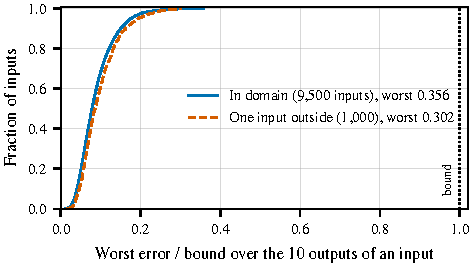
\includegraphics[width=0.6\linewidth]{fig_bound_sweep.pdf}
\caption*{Fig.~9 -- Held-out 10,500-input sweep: distribution of the worst error/bound per input.}
\end{figure}
\noindent\textbf{How to read it:} a cumulative distribution; the whole curve sits left of 0.36,
nowhere near 1. Out-of-domain inputs that were not flagged also stay inside the bound.
\say{The bound was tested on inputs the shift ranges were never fitted to; no in-domain input
raised \texttt{range\_err} and none exceeded the bound.}

\begin{figure}[H]\centering
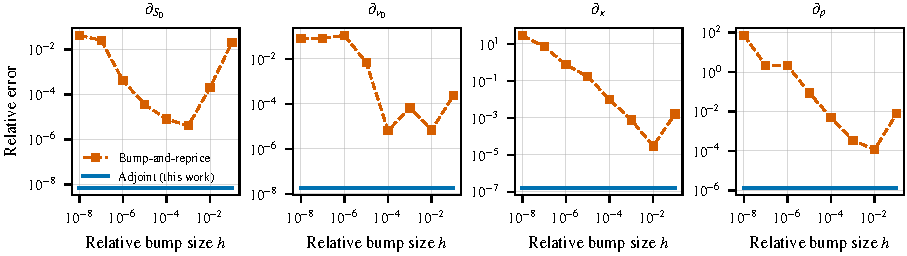
\includegraphics[width=\linewidth]{fig_bump.pdf}
\caption*{Fig.~7 -- Bump-and-reprice error against bump size, and the adjoint (flat line).}
\end{figure}
\noindent\textbf{How to read it:} U-shaped curves: on the right the truncation error of central
differences ($\propto h^2$); on the left rounding divided by $h$ ($\propto\epsilon/h$), much worse in
fixed point. The best $h$ differs per Greek; the adjoint line is below every curve.
\say{The adjoint is 32--560$\times$ more accurate (median 145$\times$) even when bump-and-reprice
gets the best bump size chosen afterwards, and it has nothing to tune.}

\begin{figure}[H]\centering
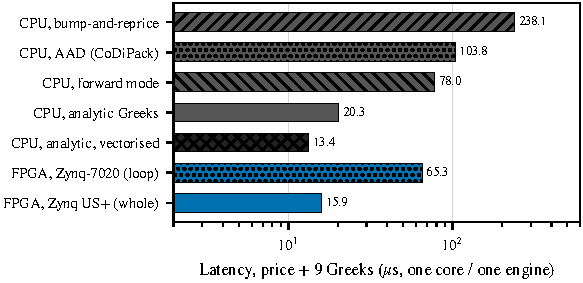
\includegraphics[width=0.62\linewidth]{fig_latency.pdf}
\caption*{Fig.~10 -- Latency of one price + 9 Greeks: one CPU core vs.\ one FPGA engine.}
\end{figure}
\noindent\textbf{How to read it:} log scale. The ZCU102 (15.9\,$\mu$s, computed) beats forward AD,
taped AAD and bumping, and scalar analytic Greeks (20.3\,$\mu$s), but \textbf{not} analytic Greeks
vectorised across terms (13.6\,$\mu$s).
\say{We are 4.9--15$\times$ faster than the general-purpose methods, but a vectorised laptop core
with hand-derived Greeks is faster than our engine, and four cores give 216,000 evaluations per
second. We claim no speed advantage over a well-optimised CPU.}

\subsection*{Tables in the paper}
I: positioning against related work. II: the three configurations. III: implementation
(LUT, FF, DSP, BRAM, clock, slack). IV: \textbf{assumptions with rationale} (A1--A14). V: adjoint
vs.\ forward mode. VI: significant figures. VII: silicon validation (1,469/1,469 bit-exact).
VIII: three equal-throughput engines (Vivado). XI: the bound relative to each value (a-priori
accuracy). XII: latency, throughput and energy vs.\ CPU, with measured CPU package power.

\subsection*{Not paper evidence}
Vivado screenshots and the hedging figures (12 NIFTY trades) are in the report only. Hedging
is an illustration: \emph{``it shows the Greeks in use, not evidence for the hardware; hedge
decisions do not depend on how the Greeks are computed.''} The old fig1--fig5 in
\texttt{validation/figures} are from the first-generation analysis and superseded.

% =====================================================================
\section{Results with the honest numbers}
\begin{center}\small
\begin{tabular}{@{}L{4.2cm}L{11.2cm}@{}}
\toprule
Greeks cost & \textbf{1.04 pricings} on the same hardware (56-bit; 1.55 on 64-bit); at equal throughput 1.03$\times$ cycles, 1.68$\times$ LUT, 2$\times$ DSP\\
vs.\ forward mode & factored forward engine: +6.8\% LUT, +12.2\% FF, +25\% DSP, 6$\times$ less accurate\\
vs.\ bump-and-reprice & 18.4$\times$ fewer cycles; 32--560$\times$ more accurate\\
Error bound & never exceeded over 10,500 + 10,500 held-out inputs (worst 0.378 / 0.356); 0.199 ZedBoard, 0.255 ZCU102\\
Accuracy (56-bit, 99th pct.) & price, delta, strike, theta, rho, vega $\ge$ 5.3 significant figures; $\partial_\kappa$ 3.5, $\partial_\xi$ 3.0\\
Silicon & ZedBoard 450/450 (+9/9 vector); ZCU102 1,010/1,010; worst ZCU102 price error $7.3\times10^{-7}$\\
Area & Zynq-7020: 72.8\% LUT, 72/220 DSP; ZCU102: 77,515 LUT (28\%), 510 DSP (20\%), +1.601\,ns at 100\,MHz\\
Latency vs.\ CPU (i5-1155G7, idle) & analytic 20.3\,$\mu$s scalar, \textbf{13.6\,$\mu$s vectorised}; ZedBoard 65.3; ZCU102 15.9 (computed): \textbf{CPU wins}; 4.9--15$\times$ faster than forward (78.0), CoDiPack (103.8), bump (238.1)\\
Throughput & 4 CPU cores 216k/s (vectorised) vs.\ one 64-bit engine 62.8k/s: \textbf{CPU wins}\\
Energy & 44\,$\mu$J (ZedBoard), 40\,$\mu$J (64-bit), simulated, chip level; CPU measured (HWiNFO): 40.9\,$\mu$J vectorised, 54.6 scalar: \textbf{parity}\\
COS method error & separate from rounding; worst vega $7.8\times10^{-3}$ ($\xi=1$, $T=0.34$); 256 terms fix it\\
\bottomrule
\end{tabular}
\end{center}
\textbf{Framing:} the contribution is the \textbf{cost and certified accuracy of Greeks in
hardware} and bit-exact silicon, not speed or energy against a CPU.

% =====================================================================
\section{Limitations and status (say these before he finds them)}
\begin{enumerate}
\item The adjoint is \textbf{hand-derived}, not generated automatically.
\item The bound is \textbf{first order} and covers \textbf{rounding only}; COS truncation error is separate and unbounded.
\item \textbf{Energy}: FPGA simulated (SAIF), CPU measured (HWiNFO): parity at chip level.
\item \textbf{No latency or throughput advantage}: a vectorised CPU core (13.6\,$\mu$s) beats the engine's computed 15.9\,$\mu$s, and four cores give 216k/s.
\item The 1.04$\times$ needs twice the multipliers of a price-only engine; at equal throughput the Greeks cost $\approx$1.7$\times$ the area.
\item The bound is a \textbf{design-time} tool (0.1\,s per input in software); the engine does not attach it to each result.
\item Bus transfers not yet timed (ZCU102 processor-system run pending).
\item Bounded input domain; $S_0$ fixed at 100 (prices scale with $(S_0,K)$ together).
\item $\partial V/\partial\kappa$ and $\partial V/\partial\xi$: about 3 significant figures at the 99th percentile.
\item Zynq-7020 timing does not close at 100\,MHz (Fmax $\approx$79; board at 70).
\item Hedging is an illustration only.
\end{enumerate}

% =====================================================================
\section{Repository map}
\begin{itemize}
\item \texttt{README.md}, \texttt{dashboard.html} -- overview and results dashboard.
\item \texttt{docs/paper/} -- the IEEE paper and its figure script; \texttt{docs/report/latex/} -- the full report; \texttt{docs/architecture.md} -- engineering notes with every number; \texttt{docs/novelty\_assessment.md} -- literature check and claim wording; \texttt{docs/greeks\_engine\_dossier.html}.
\item \texttt{hardware/gen/} -- the generator; \texttt{hardware/verilog/gen/} -- generated RTL; \texttt{hardware/sim/} -- primitive unit tests.
\item \texttt{hardware/vivado/\{zedboard, zcu104, zcu102, power\}} -- build and board scripts, SAIF power flow; \texttt{hardware/sw/\{zedboard, zcu102\}} -- ARM programs.
\item \texttt{validation/} -- \texttt{reference/} (double-precision reference), \texttt{cpu\_baseline/} (C++ and CoDiPack), sweep scripts, \texttt{results/} (every number and the board logs), \texttt{figures/}, \texttt{hedging/}.
\item \texttt{verify\_all.sh} -- \textbf{26 automated checks}, all passing. ``How do you know it is right?'' -- run it.
\end{itemize}

% =====================================================================
\section{Questions the supervisor may ask, with answers}
\subsection{Novelty and positioning}
\qa{What exactly is new?}{To our knowledge (after a literature search) the first FPGA computation of option Greeks by adjoint differentiation, and the first FPGA COS pricer (COS has run on GPUs), with (i) a co-scheduled adjoint datapath with a register-resident tape, measured against price-only and forward-mode engines of equal throughput, (ii) a per-Greek rounding bound for a fixed-point datapath that itself performs the adjoint, and (iii) bit-exact silicon on two FPGA families. Adjoints, COS and Linnainmaa's bound are each established; the combination in hardware is new.}
\qa{Is this really AAD?}{It is adjoint differentiation; the reverse sweep is hand-derived in the graph and verified. Automatic derivation is future work, and the claim is worded accordingly.}
\qa{Hasn't someone done Greeks on FPGAs?}{Yes, by re-simulation or finite differences: Klaisoongnoen et al.\ (HEART 2022, STAC-A2 Monte Carlo on an Alveo U280), the AMD Vitis Quantitative Finance library (finite differences). Capriotti \& Giles' 2024 review of fifteen years of AAD in finance lists no FPGA adjoint.}
\qa{Cui et al.\ already derived analytic Heston gradients. Why bother?}{We measured that approach: hand-derived Greeks cost 1.5 pricings on a CPU (20.3\,$\mu$s); the hardware gets 1.04 on the same hardware, 1.03$\times$ cycles and $\approx$1.7$\times$ area at equal throughput. Implemented at equal throughput, the hand-factored forward engine needs 7\% more LUTs and 25\% more DSPs and is 6$\times$ less accurate.}
\qa{Why not just use a CPU?}{For speed and energy, a CPU is as good or better: vectorised analytic Greeks take 13.6\,$\mu$s on one core and the energy per evaluation is at parity. The FPGA's case is the cost and accuracy of its Greeks in hardware, a first-order bound on every Greek, deterministic latency, and a datapath that a generator produces and verifies automatically.}
\qa{Delta and Gamma come almost free from the COS sum. Isn't the adjoint overkill?}{Yes for Delta and the strike sensitivity (closed forms, Fang \& Oosterlee Remark 3.2); the adjoint's real work is the seven Greeks entering through the characteristic function. A fair bump baseline using the closed forms needs 15 pricings ($\approx$14.5$\times$ the adjoint's cycles, not 18.4). Gamma is second order and not computed.}

\subsection{Heston and COS}
\qa{Which characteristic-function form, and why?}{The stable form (Albrecher et al.), $g=(\kappa-i\rho\xi u-d)/(\kappa-i\rho\xi u+d)$ with $e^{-dT}$; it avoids the branch-cut discontinuity of the complex logarithm for long maturities.}
\qa{How did you choose $N=128$ and the range?}{Standard COS choices (cumulant range, $\pm$10 standard deviations). The method-error study shows typical errors around $10^{-9}$--$10^{-11}$, with a few hard cases (high $\xi$ with short $T$; deep out-of-the-money puts) where 256 terms or a 1.5$\times$ wider range is needed.}
\qa{You freeze $[a,b]$ when differentiating. Is that valid?}{The Greeks are exact derivatives of the COS approximation at a fixed range. The range's dependence on the parameters only affects the truncated tails and vanishes with the truncation error; the reference uses the same convention, and the Greeks were compared with an independent Fourier-integral reference.}
\qa{Why puts with parity instead of calls?}{Call payoff coefficients contain $e^{b}$ and cancel catastrophically in fixed point; parity moves that to one exact correction. Worst call price error fell 75$\times$.}
\qa{What about the Feller condition?}{COS does not need it; the 10,500-input sweep has a Feller-violation regime and the bound held there.}
\qa{Your vega is $\partial V/\partial v_0$. Is that standard?}{It is with respect to variance; $\partial V/\partial\sigma_0 = 2\sigma_0\,\partial V/\partial v_0$, a one-line conversion.}
\qa{Why is $S_0$ fixed?}{Homogeneity: $V(\lambda S_0,\lambda K)=\lambda V(S_0,K)$. The host scales inputs and outputs.}

\subsection{Adjoint differentiation}
\qa{Where is the tape?}{In registers. The schedule is static, so each forward value's lifetime is known; the scheduler keeps it in a rotating register until the reverse sweep uses it: 447 across all terms in flight, against 150 for a price-only schedule. It costs flip-flops (and some shift-register LUTs), not memory traffic.}
\qa{Why reverse mode with only 9 inputs?}{Reverse costs about one sweep per output: one output, nine inputs. The forward-mode table quantifies it: 250 multiplies per term against 313--802.}
\qa{The cheap-gradient bound is 4--5$\times$. How do you get 1.04?}{In operations it is 250/126 $\approx$ 2$\times$ multiplies; in \emph{time} it is 1.04 on the same hardware because the CORDIC units set the pace and the adjoint's multiplies fill idle multiplier slots. But a price-only engine needs only half the multipliers for that pace, so in area-time the Greeks cost about 2$\times$ multipliers, 1.7$\times$ area. Where multipliers bind (64-bit) it is 1.55$\times$ on the same hardware.}
\qa{How did you verify the adjoint?}{Against the double-precision model and the forward-mode datapaths ($6\times10^{-14}$), against CoDiPack and analytic Greeks on the CPU ($1.3\times10^{-10}$), and bit-exact RTL against the emulator.}

\subsection{Fixed point and the bound}
\qa{Derive your bound.}{Each operation adds a rounding error of at most $\tfrac12$ ulp; to first order the output error is $\sum_i (\partial y/\partial w_i)\,\delta_i$; bound each term by its absolute value: $\sum_i |\partial y/\partial w_i|\,2^{-(FL+1)}$. The sensitivities come from a reverse sweep over the graph (Linnainmaa 1976).}
\qa{Why only first order?}{Second-order terms are $\approx2^{-28}$ smaller. Checked: 50-digit evaluation agrees ($\le$ 0.24 of the bound), and the bound holds at 44 bits where those terms are 4,096$\times$ larger.}
\qa{Is it a rigorous bound?}{A first-order estimate, not interval arithmetic; rigorous up to the dropped second-order terms, which the checks show are negligible. Say ``first-order bound'', never ``guaranteed''. AD-based word-length analysis on FPGAs is prior art (Gaffar et al.\ 2002; Lee et al.\ 2006); our step is applying it to a datapath that contains its own adjoint.}
\qa{How are CORDIC, Newton--Raphson and tables modelled in the bound?}{Newton--Raphson, tables and series are expanded into graph operations, so each internal rounding is modelled; their approximation error is common to the fixed and exact evaluations and is $\le1.1\times10^{-8}$ relative. CORDIC units are single operations with measured local errors: rotation $\le$1.14\,ulp (modelled 2); the vectoring angle grows as $1.75/|z|$\,ulp, so it is modelled as $2\max(1,1/|z|)$\,ulp. That correction was found during the review; no published number changed.}
\qa{Why is the bound loose (0.1--0.4)?}{Worst-case half-ulp errors with aligned signs do not happen; rounding errors partly cancel. 0.1--0.4 is tight for a worst-case bound.}
\qa{Why 56 bits?}{The shortest word at which every Greek's worst relative error is $\le1.2\times10^{-5}$ on the grid (52 bits: $5.8\times10^{-4}$), with the error under the bound; and 56$\times$56 maps to 9 DSP48s. The 64-bit design is for the larger chip.}
\qa{How do you prevent overflow?}{Shift ranges measured over the domain plus margin; every shifter raises \texttt{range\_err} if exceeded. No overflows over 10,500 inputs; flags only outside the domain after the refit.}
\qa{Isn't refitting ranges on test data overfitting?}{That is why there is a held-out sweep (seed 20261006, 10,500 new inputs): no in-domain flags, worst bound ratio 0.356.}

\subsection{Hardware}
\qa{Explain modulo scheduling and your II.}{Iterations (terms) start every II cycles and overlap; II is at least the resource bound: $\lceil250/8\rceil=32$ for multipliers and 32 for the CORDIC units too. Loop = $(N-1)\cdot$II + latency = $127\cdot32+506+2=4{,}572$.}
\qa{Why no dividers?}{Newton--Raphson reciprocals and square roots reuse the multipliers; Tang's exponential, a table-plus-series log and CORDIC (trig, complex magnitude/angle) keep everything on the shared units.}
\qa{Why CORDIC rather than DSP-based sin/cos?}{CORDIC uses no DSPs (shift-add) and its fixed iteration count suits a static schedule; the price is that it sets the II.}
\qa{Why doesn't the Zynq-7020 close 100\,MHz?}{The 56-bit carry chains; Vivado suggests using the DSP blocks' internal pipeline registers (future work). UltraScale+ meets 100\,MHz with +1.6\,ns.}
\qa{How many resources does the adjoint add?}{Same II, same 8 multipliers; extra registers hold forward values for the reverse sweep; still fits the Zynq-7020 (73\% LUT).}
\qa{How is it verified end to end?}{Primitives unit-tested; RTL checked per register against the emulator; wrappers bit-exact; board outputs bit-exact against the emulator, so every model-level accuracy result transfers to silicon. \texttt{verify\_all.sh} runs 26 checks.}
\qa{Did you simulate the gate-level netlist?}{Yes, for power: the routed netlists were simulated on 4 evaluations, bit-exact, and the activity fed into Vivado's power analysis (SAIF).}

\subsection{Results and fairness}
\qa{Is the CPU comparison fair?}{Same algorithm (COS 128, frozen range, parity) in double precision, g++ -O3 -march=native, best of 5 on an idle machine, and the strongest software baseline (hand-derived analytic Greeks) included. The ZedBoard figure is loop-only (the CPU's work outside its loop is 0.03\,$\mu$s); bus transfers are not yet timed.}
\qa{Your energy numbers?}{FPGA: simulated activity on the routed netlist, chip level (2.485\,W $\times$ 15.9\,$\mu$s $\approx$ 40\,$\mu$J). CPU: package power measured with HWiNFO, 8.8\,W with eight processes at 216,000/s $\approx$ 40.9\,$\mu$J. Parity, so no energy claim.}
\qa{Throughput is worse than 4 cores. Why should anyone care?}{We do not claim throughput. Three engines would fit on the ZCU102 by LUTs ($\approx$188k/s, projected), still below the vectorised CPU's 216k/s. The case is the cost and certified accuracy of the Greeks.}
\qa{Did you compare against a vectorised CPU?}{Yes: the \texttt{-O3} loop was scalar; a structure-of-arrays version with glibc's vector maths takes 13.6\,$\mu$s on one core and beats the engine's computed latency. A single-loop vectorised version spilled registers and was slower than scalar.}
\qa{Only 21 cases for the accuracy figure?}{Fig.~8 shows 21 for readability; the claim rests on 10,500 + 10,500 held-out inputs including seven hard regimes, plus a 50-digit check.}
\qa{Why are $\partial V/\partial\kappa$ and $\partial V/\partial\xi$ weak?}{They are small and computed through long chains with cancellation. Always within their bound, and the bound tells the user their accuracy in advance; that is the point of a bound.}

\subsection{Practicalities and status}
\qa{What happened with the ZCU102 processor run?}{The board's DDR fails calibration with Vivado's preset (likely a different memory module on the lab board's revision). The program now runs from on-chip memory and the setup skips the DDR steps; the re-run is pending.}
\qa{Why the NIFTY data?}{To test silicon on real calibrated parameters, not only random draws: 50 trading days, all bit-exact on the ZCU102.}
\qa{Does the hedging show your Greeks are better?}{No, and we do not claim that; it is an illustration with 12 trades.}
\qa{What's next?}{Finish the ZCU102 processor-system run (end-to-end latency, board power); automatic derivation of the reverse sweep; several engines per device; 100\,MHz on the Zynq-7020 with DSP pipeline registers; strike chains (one reverse sweep serves every strike; designed and scheduled, not built).}

% =====================================================================
\section{Last-minute advice}
\begin{itemize}
\item If he challenges a number, answer from \texttt{validation/results/} and the paper's tables.
\item \textbf{Lead with the honest limits} (hand-derived adjoint; first-order, design-time bound; no speed or energy advantage over a vectorised CPU; the Greeks cost $\approx$1.7$\times$ the area at equal throughput) before he finds them.
\item The three sentences to remember:
\begin{enumerate}
\item \emph{``The reverse sweep is co-scheduled with the forward pass; its tape lives in scheduled registers.''}
\item \emph{``At equal throughput the Greeks cost 3\% in cycles and about 1.7$\times$ the area, less than forward mode, and 6$\times$ more accurate.''}
\item \emph{``Every Greek has a first-order rounding bound, never exceeded in 21,000 inputs or on silicon.''}
\end{enumerate}
\end{itemize}
\end{document}
